% Afficher des recommendations concernant la syntaxe.
\RequirePackage[orthodox,l2tabu]{nag}
\RequirePackage{luatex85}
% Paramètres du document.
\documentclass[%
a6paper%                       Taille de page.
,fontsize=8pt%                 Taille de police.
,DIV=13%                       Plus grand => des marges plus petites.
,titlepage=on%                 Faut-il une page de titre ?
,headings=optiontoheadandtoc%  Effet des paramètres optionnels de section.
,headings=small%
,parskip=false%
]{scrbook}

% Par souci de clarté, la définition des commandes est reportée dans un document annexe.
\usepackage{gredoc}
\usepackage{etoolbox}
\makeatletter
\patchcmd{\scr@startchapter}{\if@openright\cleardoublepage\else\clearpage\fi}{}{}{}
\makeatother

\title{Complies}
\date{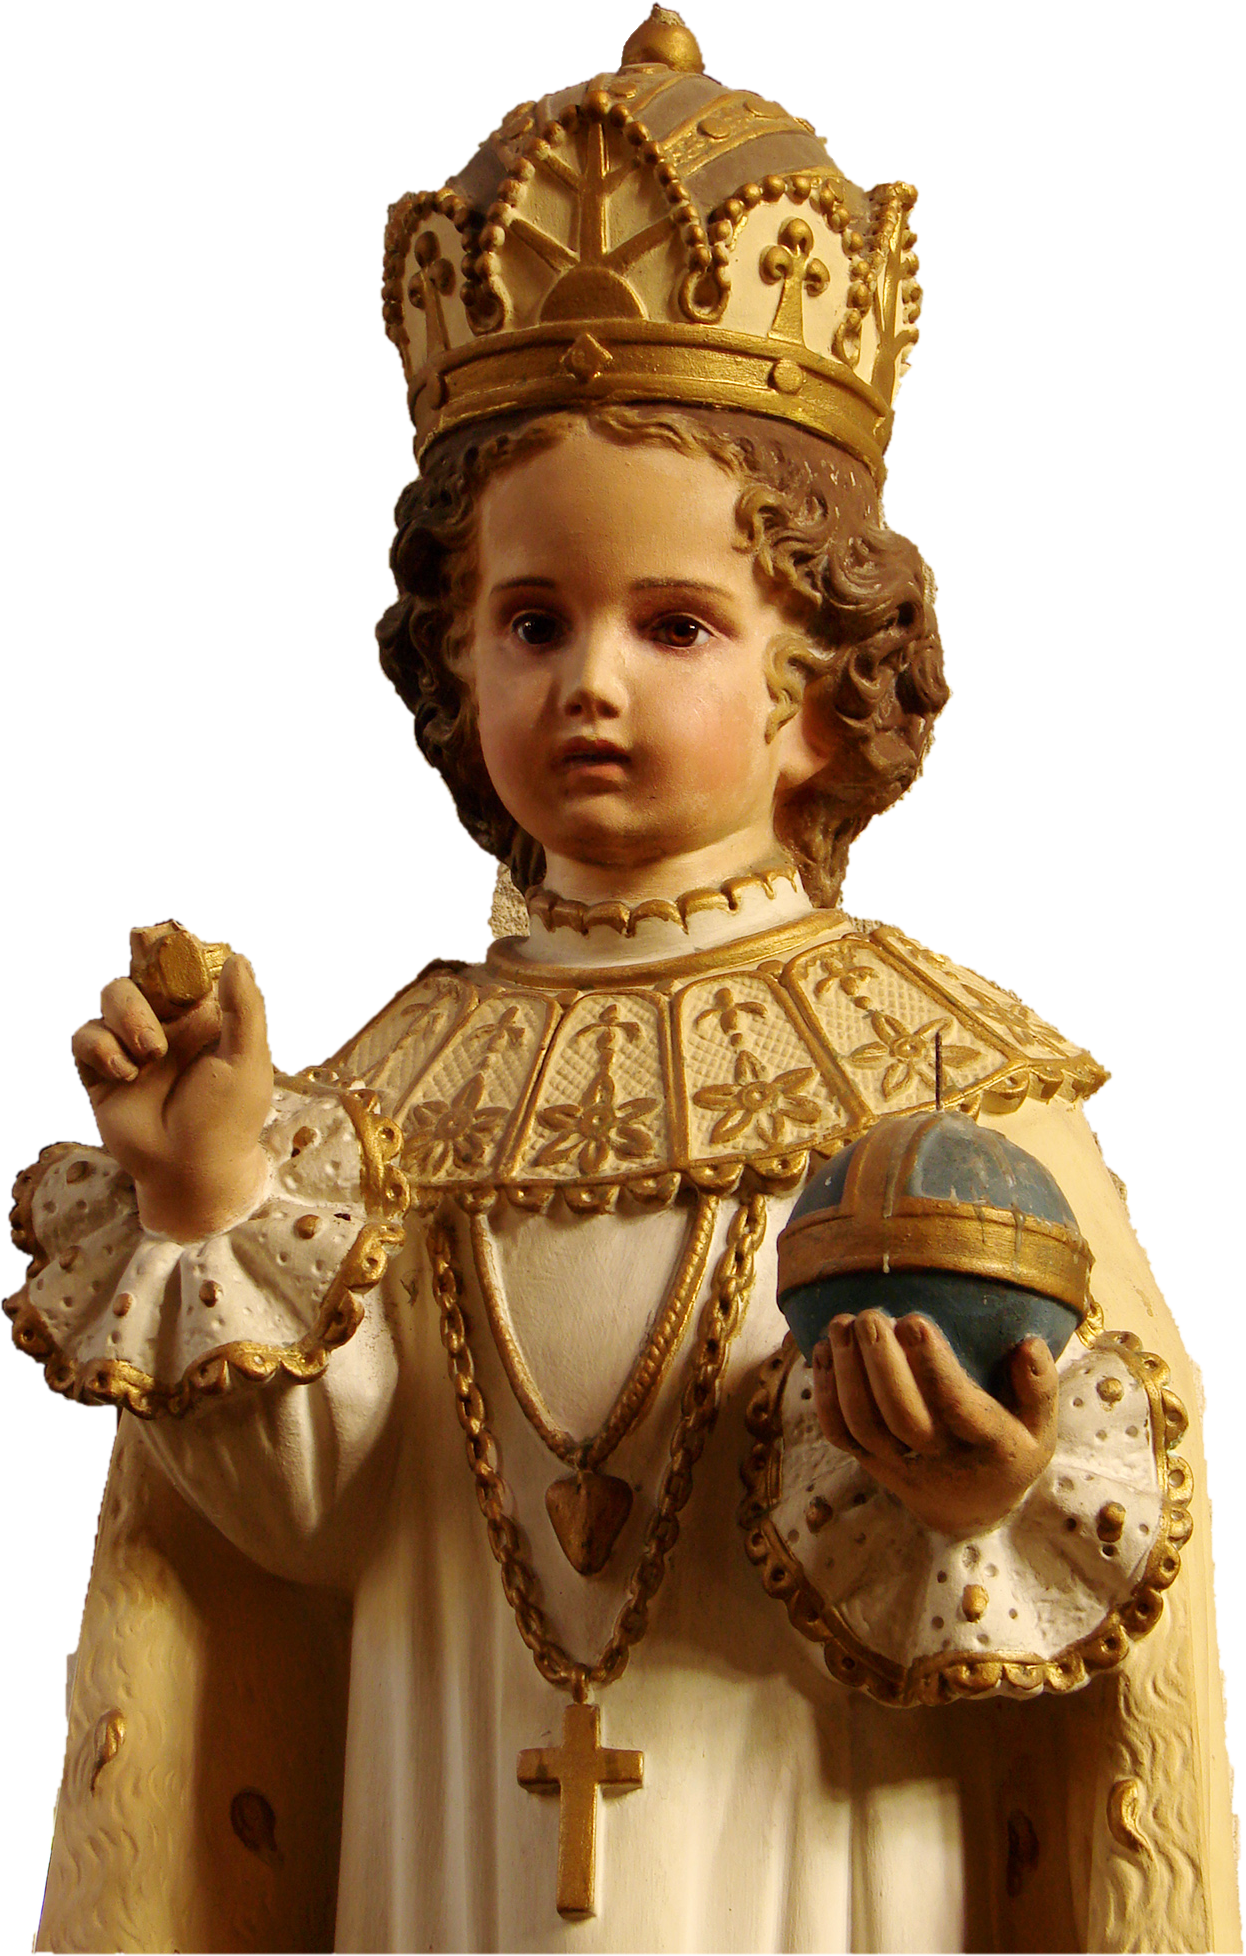
\includegraphics[height=.4\paperheight]{Couverture}}


\begin{document}

\maketitle

\backmatter
\setcounter{page}{1}\tableofcontents


\part{Complies}

\chapter{Leçon brève et Confíteor}

\section{Leçon brève}

\rubrica[french]{On commence les complies debout. Le chantre entonne%
\footnote{En l'absence de prêtre ou de diacre : \emph{Iube \textbf{Dómine} benedícere.}} :}
\smallskip

\label{IubeDomne}
\cantus[0]{Verset}{IubeDomne}{}{}

\cantus[0]{Verset}{NoctemQuietam}{}{}

\cantus{Lecon}{FratresSobrii}{}{}

\cantus[0]{Verset}{AdiutoriumNostrum}{}{}%

\rubrica[french]{\emph{\color{black} Pater noster} tout bas en entier.}

\section{Confíteor}

\label{Confiteor}
\rubrica[french]{Le célébrant, profondément incliné, récite le \emph{\color{black} Confíteor}\footnotemark.}%
\footnotetext{%
En l'absence de prêtre ou de diacre, tous récitent en même temps le \emph{Confíteor}, modifié comme suit :

\emph{Confíteor Deo omnipoténti, beátæ Maríæ semper Vírgini, beáto Michaéli Archángelo, beáto Ioánni Baptístæ, sanctis Apóstolis Petro et Paulo, et ómnibus Sanctis : quia peccávi nimis cogitatióne, verbo et ópere: mea culpa, mea culpa, mea máxima culpa. Ideo precor beátam Maríam semper Vírginem, beátum Michaélem Archángelum, beátum Ioánnem Baptístam, sanctos Apóstolos Petrum et Paulum, et omnes Sanctos, oráre pro me ad Dóminum Deum nostrum.}

\noindent Le "célébrant" dit alors :

\emph{Misereátur nostri omnípotens Deus, et, dimíssis peccátis nostris, perdúcat nos ad vitam ætérnam. ℟. Amen.}

\emph{Indulgéntiam, absolutiónem, et remissiónem peccatórum nostrórum tríbuat nobis omnípotens et miséricors Dóminus. ℟. Amen.}%
}

\rubrica[french]{Le chœur répond en s'inclinant profondément :}%


Misereátur tui omnípotens Deus, et, dimíssis peccátis tuis, perdúcat te ad vitam ætérnam. ℟. Amen.

Confíteor Deo omnipoténti, beátæ Maríæ semper Vírgini, beáto Michaéli Archángelo, beáto Ioánni Baptístæ, sanctis Apóstolis Petro et Paulo, ómnibus Sanctis, et tibi, pater : quia peccávi nimis cogitatióne, verbo et ópere: mea culpa, mea culpa, mea máxima culpa. Ideo precor beátam Maríam semper Vírginem, beátum Michaélem Archángelum, beátum Ioánnem Baptístam, sanctos Apóstolos Petrum et Paulum, omnes Sanctos, et te, pater, oráre pro me ad Dóminum Deum nostrum.

\rubrica[french]{Le célébrant :}

Misereátur vestri omnípotens Deus, et, dimíssis peccátis vestris, perdúcat vos ad vitam ætérnam. ℟. Amen.

Indulgéntiam, absolutiónem, et remissiónem peccatórum nostrórum tríbuat nobis omnípotens et miséricors Dóminus. ℟. Amen.
\medskip

\cantus[0]{Verset}{ConverteNos}{}{}

\label{DeusInAdiutorium}
\cantus[0]{Verset}{DeusInAdiutorium}{}{}


\chapter{Antiennes et Psaumes}

\rubrica[french]{Les antiennes et psaumes varient en fonction du jour de la semaine ; mais pour les fêtes de I\iere\ et II\ieme\ classes, on prend les antiennes et psaumes du dimanche.}

\rubrica[french]{Avant les psaumes, le célébrant entonne l'antienne, que le chœur reprend à partir de l'étoile. Le chantre entonne le premier verset de chaque psaume, et les psaumes sont alternés entre les deux moitiés du chœur ; à la fin, tous reprennent ensemble l'antienne.
On s'assied après l'intonation du premier psaume.}

\bigskip
\rubrica[french]{Au Temps pascal, l'antienne est toujours la même :}

\medskip
\cantus{Antienne}{Alleluia}{Ant.}{8G.}


\needspace{.6\paperwidth}
\section{Dimanche}\label{Dimanche}\paginarectavacua

\cantus{Antienne}{Miserere}{Ant.}{8G.}

\ps{IV}
\cantus[0]{Psaume}{Intonation-004-8G}{}{}
\psalmus[%
tonus=8G,%
primus=2,numerus=2,%
ultimus=10,%
]{004}
\gloria[tonus=8G]

\ps{XC}
\cantus[0]{Psaume}{Intonation-090-8G}{}{}
\psalmus[%
tonus=8G,%
primus=2,numerus=2,%
ultimus=16,%
]{090}
\gloria[tonus=8G]

\vspace{-.5\baselineskip plus .5\baselineskip}
\ps{CXXXIII}
\cantus[0]{Psaume}{Intonation-133-8G}{}{}
\psalmus[%
tonus=8G,%
primus=2,numerus=2,%
ultimus=4,%
]{133}
\gloria[tonus=8G]

\vspace{-.5\baselineskip plus .5\baselineskip}
\medskip
\cantus{Antienne}{Miserere}{Ant.}{8G.}

\medskip
\rubrica[french]{L'Office se poursuit par le chant du \emph{\color{black}Te lucis}, p.\,\pageref{TeLucis} et suivantes.}\pagebreak[3]


\needspace{.6\paperwidth}
\section{Lundi}\label{Lundi}\paginarectavacua

\cantus{Antienne}{SalvumMeFac}{Ant.}{8G.}

\ps{VI}
\cantus[0]{Psaume}{Intonation-006-8G}{}{}
\smallskip
\psalmus[%
tonus=8G,%
primus=2,numerus=2,%
ultimus=10,%
]{006}
\gloria[tonus=8G]

\smallskip
\ps{VII. 1}
\cantus[0]{Psaume}{Intonation-007-01-8G}{}{}
\smallskip
\psalmus[%
tonus=8G,%
primus=2,numerus=2,%
ultimus=10,%
]{007}
\gloria[tonus=8G]

\smallskip
\ps{VII. 2}
\cantus[0]{Psaume}{Intonation-007-11-8G}{}{}
\smallskip
\psalmus[%
tonus=8G,%
primus=12,numerus=2,%
ultimus=18,%
]{007}
\gloria[tonus=8G]

\medskip
\cantus{Antienne}{SalvumMeFac}{Ant.}{8G.}

\medskip
\rubrica[french]{L'Office se poursuit par le chant du \emph{\color{black}Te lucis}, p.\,\pageref{TeLucis} et suivantes.}\pagebreak[3]


\needspace{.6\paperwidth}
\section{Mardi}\label{Mardi}\paginarectavacua

\cantus{Antienne}{TuDomine}{Ant.}{8G.}

\ps{XI}
\cantus[0]{Psaume}{Intonation-011-8G}{}{}
\psalmus[%
tonus=8G,%
primus=2,numerus=2,%
ultimus=9,%
]{011}
\gloria[tonus=8G]

\ps{XII}
\cantus[0]{Psaume}{Intonation-012-8G}{}{}
\smallskip
\psalmus[%
tonus=8G,%
primus=2,numerus=2,%
ultimus=6,%
]{012}
\gloria[tonus=8G]

\ps{XV}
\cantus[0]{Psaume}{Intonation-015-8G}{}{}
\smallskip
\psalmus[%
tonus=8G,%
primus=2,numerus=2,%
ultimus=11,%
]{015}
\gloria[tonus=8G]

\medskip
\cantus{Antienne}{TuDomine}{Ant.}{8G.}

\medskip
\rubrica[french]{L'Office se poursuit par le chant du \emph{\color{black}Te lucis}, p.\,\pageref{TeLucis} et suivantes.}\pagebreak[3]


\needspace{.6\paperwidth}
\section{Mercredi}\label{Mercredi}\paginarectavacua

\cantus{Antienne}{Immitet}{Ant.}{3a.}

\ps{XXXIII. 1}
\cantus[0]{Psaume}{Intonation-033-01-3a}{}{}
\rubrica[french]{Au Temps pascal :}

\cantus[0]{Psaume}{Intonation-033-01-8G}{}{}
\smallskip
\psalmus[%
tonus=3a,%
primus=2,numerus=2,%
ultimus=10,%
]{033}
\gloria[tonus=3a]

\ps{XXXIII. 2}
\cantus[0]{Psaume}{Intonation-033-11-3a}{}{}
\rubrica[french]{Au Temps pascal :}

\cantus[0]{Psaume}{Intonation-033-11-8G}{}{}
\smallskip
\psalmus[%
tonus=3a,%
primus=12,numerus=2,%
ultimus=22,%
]{033}
\gloria[tonus=3a]

\ps{LX}
\cantus[0]{Psaume}{Intonation-060-3a}{}{}
\rubrica[french]{Au Temps pascal :}

\cantus[0]{Psaume}{Intonation-060-8G}{}{}
\smallskip
\psalmus[%
tonus=3a,%
primus=2,numerus=2,%
ultimus=8,%
]{060}
\gloria[tonus=3a]

\medskip
\cantus{Antienne}{Immitet}{Ant.}{3a.}

\medskip
\rubrica[french]{L'Office se poursuit par le chant du \emph{\color{black}Te lucis}, p.\,\pageref{TeLucis} et suivantes.}\pagebreak[3]


\needspace{.6\paperwidth}
\section{Jeudi}\label{Jeudi}\paginarectavacua

\cantus{Antienne}{AdiutorMeus}{Ant.}{8G.}

\ps{LXIX}
\cantus[0]{Psaume}{Intonation-069-8G}{}{}
\smallskip
\psalmus[%
tonus=8G,%
primus=2,numerus=2,%
ultimus=7,%
]{069}
\gloria[tonus=8G]

\smallskip
\ps{LXX. 1}
\cantus[0]{Psaume}{Intonation-070-01-8G}{}{}
\smallskip
\psalmus[%
tonus=8G,%
primus=2,numerus=2,%
ultimus=13,%
]{070}
\gloria[tonus=8G]

\smallskip
\ps{LXX. 2}
\cantus[0]{Psaume}{Intonation-007-14-8G}{}{}
\psalmus[%
tonus=8G,%
primus=15,numerus=2,%
ultimus=26,%
]{070}
\gloria[tonus=8G]

\medskip
\cantus{Antienne}{AdiutorMeus}{Ant.}{8G.}

\medskip
\rubrica[french]{L'Office se poursuit par le chant du \emph{\color{black}Te lucis}, p.\,\pageref{TeLucis} et suivantes.}\pagebreak[3]


\needspace{.6\paperwidth}
\section{Vendredi}\label{Vendredi}\paginarectavacua

\cantus{Antienne}{VoceMea}{Ant.}{7c.}

\ps{LXXVI. 1}
\cantus[0]{Psaume}{Intonation-076-1-7c}{}{}
\rubrica[french]{Au Temps pascal :}

\cantus[0]{Psaume}{Intonation-076-1-8G}{}{}
\smallskip
\psalmus[%
tonus=7c,%
primus=2,numerus=2,%
ultimus=12,%
]{076}
\gloria[tonus=7c]

\smallskip
\ps{LXXVI. 2}
\cantus[0]{Psaume}{Intonation-076-13-7c}{}{}
\rubrica[french]{Au Temps pascal :}

\cantus[0]{Psaume}{Intonation-076-13-8G}{}{}
\smallskip
\psalmus[%
tonus=7c,%
primus=14,numerus=2,%
ultimus=20,%
]{076}
\gloria[tonus=7c]

\smallskip
\ps{LXXXV}
\cantus[0]{Psaume}{Intonation-085-7c}{}{}
\rubrica[french]{Au Temps pascal :}

\cantus[0]{Psaume}{Intonation-085-8G}{}{}
\smallskip
\psalmus[%
tonus=7c,%
primus=2,numerus=2,%
ultimus=16,%
]{085}
\gloria[tonus=7c]

\medskip
\cantus{Antienne}{VoceMea}{Ant.}{7c.}

\medskip
\rubrica[french]{L'Office se poursuit par le chant du \emph{\color{black}Te lucis}, p.\,\pageref{TeLucis} et suivantes.}\pagebreak[3]


\needspace{.6\paperwidth}
\section{Samedi}\label{Samedi}\paginarectavacua

\cantus{Antienne}{IntretOratioMea}{Ant.}{5a.}

\ps{LXXXVII}
\cantus[0]{Psaume}{Intonation-087-5a}{}{}
\rubrica[french]{Au Temps pascal :}

\cantus[0]{Psaume}{Intonation-087-8G}{}{}
\smallskip
\psalmus[%
tonus=5a,%
primus=2,numerus=2,%
ultimus=19,%
]{087}
\gloria[tonus=5a]

\smallskip
\ps{CII. 1}
\cantus[0]{Psaume}{Intonation-102-1-5a}{}{}
\rubrica[french]{Au Temps pascal :}

\cantus[0]{Psaume}{Intonation-102-1-8G}{}{}
\smallskip
\psalmus[%
tonus=5a,%
primus=2,numerus=2,%
ultimus=12,%
]{102}
\gloria[tonus=5a]

\vspace{0ex plus 1ex minus 1ex}
\ps{CII. 2}
\cantus[0]{Psaume}{Intonation-102-13-5a}{}{}
\rubrica[french]{Au Temps pascal :}

\cantus[0]{Psaume}{Intonation-102-13-8G}{}{}
\smallskip
\psalmus[%
tonus=5a,%
primus=14,numerus=2,%
ultimus=22,%
]{102}
\gloria[tonus=5a]

\medskip
\cantus{Antienne}{IntretOratioMea}{Ant.}{5a.}

\smallskip
\rubrica[french]{L'Office se poursuit par le chant du \emph{\color{black}Te lucis}, p.\,\pageref{TeLucis} et suivantes.}\pagebreak[3]


\clearpage
\chapter{Hymne}\label{TeLucis}

\rubrica[french]{La reprise de l'antienne achevée, le chœur se lève pour le chant de l'hymne. Le ton de l'hymne \emph{\color{black}Te lucis} varie en fonction des temps de l'année ; l'hymne achevé, on poursuit par le capitule, p.\pageref{capitule}.}

\section[Dimanches de l'année]{Dimanches de l'année \small et fêtes de II\ieme\ ou III\ieme\ classes}

\cantus{Hymne}{TeLucis}{}{8.}

\section[Féries de l'année]{Féries du temps après la Pentecôte\\et du 14 janvier au Carême}\paginarectavacua

\cantus{Hymne}{TeLucis-Ferial}{}{4.}

\section{Fêtes de I\iere\ classe}\paginarectavacua

\cantus{Hymne}{TeLucis-Solennel}{}{4.}

\section{Avent}\paginarectavacua

\cantus{Hymne}{TeLucis-Avent}{}{2.}

\section{Temps de Noël et Fête-Dieu}\paginarectavacua

\cantus{Hymne}{TeLucis-Noel}{}{2.}

\section{Temps de l'Épiphanie}\paginarectavacua

\cantus{Hymne}{TeLucis-Epiphanie}{}{8.}

\section{Sainte Famille}\paginarectavacua

\cantus{Hymne}{TeLucis-SteFamille}{}{8.}

\needspace{.3\paperheight}
\section{Carême}\paginarectavacua

\rubrica[french]{Ce ton s'utilise de la veille du I\ier\ dimanche de Carême à l'avant-veille du dimanche de la Passion inclusivement.}

\smallskip
\cantus{Hymne}{TeLucis-Careme}{}{2.}

\section{Temps de la Passion}\paginarectavacua

\cantus{Hymne}{TeLucis-Passion}{}{2.}

\section{Dimanches et fêtes du Temps pascal}\paginarectavacua

\cantus{Hymne}{TeLucis-TP}{}{8.}

\section{De l'Ascension à la Pentecôte}\paginarectavacua

\cantus{Hymne}{TeLucis-Ascension}{}{4.}

\section{Pentecôte et son octave}\paginarectavacua

\cantus{Hymne}{TeLucis-Pentecote}{}{1.}

\section*{Fête-Dieu : comme à Noël}\paginarectavacua

\section{Sacré-Cœur}\paginarectavacua

\cantus{Hymne}{TeLucis-SacreCoeur}{}{3.}

\section{Transfiguration}\paginarectavacua

\cantus{Hymne}{TeLucis-Transfiguration}{}{4.}

\section{Christ-Roi}\paginarectavacua

\cantus{Hymne}{TeLucis-ChristRoi}{}{1.}

\section{Notre-Dame des sept Douleurs}\paginarectavacua

\cantus{Hymne}{TeLucis-SeptDouleurs}{}{2.}

\section[Fêtes de la sainte Vierge]{Autres fêtes de Notre-Dame}\paginarectavacua

\cantus{Hymne}{TeLucis-SteVierge}{}{2.}



\chapter{Capitule et répons bref}

\section{Capitule}\label{capitule}

\cantus{Autre}{TuAutemInNobisEs}{}{}

\needspace{.1\paperheight}
\section{\mbox{Répons bref}}

\subsection{Pendant l'année}

\cantus{Repons}{InManus}{}{6.}

\rubrica[french]{Du samedi de \emph{Sitientes} au Mercredi~Saint inclus, on omet \emph{\color{black}Glória Patri, et Fílio, et Spirítui Sancto}, et on reprend directement \emph{\color{black}In manus.}}

\medskip
\cantus[0]{Verset}{CustodiNos}{}{}

\subsection{Pendant l'Avent}
\cantus{Repons}{InManus-Avent}{}{4.}
\cantus[0]{Verset}{CustodiNos-Avent}{}{}

\subsection{Au Temps pascal}
\cantus{Repons}{InManus-TP}{}{6.}
\cantus[0]{Verset}{CustodiNos-TP}{}{}


\chapter{Nunc dimíttis}

\rubrica[french]{Le célébrant entonne l'antienne :}

\smallskip
\cantus{Antienne}{SalvaNos}{Ant.}{3.}

\rubrica[french]{Le chantre entonne le psaume :}

\label{NuncDimittis}
\cantus[0]{Psaume}{NuncDimittis-3a}{}{}
\cantus{Antienne}{SalvaNos}{Ant.}{3.}


\chapter{Oraison et conclusion}

\rubrica[french]{Si le célébrant n'est pas prêtre ni diacre, il ne dit jamais \emph{Dóminus vobíscum}, mais il dit à la place : \emph{\color{black} Dómine, exáudi oratiónem meam.}}

\medskip\label{VisitaQuaesumus}
\cantus[0]{Verset}{DominusVobiscum-simple}{}{}
\cantus{Autre}{VisitaQuæsumus}{}{}

\cantus[0]{Verset}{DominusVobiscum-simple}{}{}

\cantus[0]{Verset}{BenedicamusDomino-complies}{}{}

\rubrica[french]{Le célébrant chante alors \emph{recto tono} et sur un ton un peu bas :}

Benedícat et custódiat nos omnípotens et miséricors Dóminus, Pater, et Fílius, et Spíritus Sanctus.
℟. Amen.


\chapter{Antienne à Notre-Dame}

\rubrica[french]{On chante, en fonction du temps liturgique, l'une des antiennes à la Sainte Vierge, entonnée par le célébrant. On chante le ton solennel les dimanches et fêtes de première ou deuxième classe, le ton simple les autres jours. On se tient debout le samedi et le dimanche ainsi qu'au Temps pascal, à genoux les autres jours.}


\section{\mbox{Alma Redemptóris}}

\rubrica[french]{De la veille du 1\ier\ dimanche de l'Avent au 1\ier\ février inclus.}

\subsection{Ton solennel}

\cantus{Antienne}{Alma-solennel}{Ant.}{5.}

\subsection{Ton simple}

\cantus{Antienne}{Alma-simple}{Ant.}{5.}

\subsection{Verset et oraison}

\rubrica[french]{Pendant l'Avent :}

\smallskip
\cantus[0]{Verset}{AngelusDomini}{}{}
\cantus{Autre}{GratiamTuam}{}{}

\rubrica[french]{De la vigile de Noël au 1\ier\ février inclus :}

\smallskip
\cantus[0]{Verset}{PostPartum}{}{}
\cantus{Autre}{DeusQuiSalutis}{}{}

\rubrica[french]{Le célébrant conclut, \emph{recto tono} sur un ton un peu bas :}

℣. Divínum auxílium máneat semper nobíscum. ℟. Amen.


\section{Ave Regína cælórum}

\rubrica[french]{Du 2 février inclus aux complies du Mercredi de la Semaine Sainte.}

\subsection{Ton solennel}

\cantus{Antienne}{AveReginaCaelorum-solennel}{Ant.}{6.}

\subsection{Ton simple}

\cantus{Antienne}{AveReginaCaelorum-simple}{Ant.}{6.}

\subsection{Verset et oraison}

\cantus[0]{Verset}{DignareMeLaudare}{}{}

\cantus{Autre}{ConcedeMisericorsDeus}{}{}

\rubrica[french]{Le célébrant conclut, \emph{recto tono} sur un ton un peu bas :}

℣. Divínum auxílium máneat semper nobíscum. ℟. Amen.


\needspace{.4\paperheight}
\section{Regína cæli}

\rubrica[french]{Du dimanche de Pâques au vendredi après la Pentecôte inclus.}

\subsection{Ton solennel}

\cantus{Antienne}{ReginaCaeli-solennel}{Ant.}{6.}

\subsection{Ton simple}

\cantus{Antienne}{ReginaCaeli-simple}{Ant.}{6.}

\subsection{Verset et oraison}

\cantus[0]{Verset}{GaudeEtLaetare}{}{}

\cantus{Autre}{DeusQuiPerResurrectionem}{}{}

\rubrica[french]{Le célébrant conclut, \emph{recto tono} sur un ton un peu bas :}

℣. Divínum auxílium máneat semper nobíscum. ℟. Amen.


\needspace{.3\paperheight}
\section{Salve Regína}

\rubrica[french]{De la fête de la Sainte Trinité jusqu'au vendredi avant le 1\ier\ dimanche de l'Avent inclus.}

\subsection{Ton solennel}

\cantus{Antienne}{SalveRegina-solennel}{Ant.}{1.}

\subsection{Ton simple}

\cantus{Antienne}{SalveRegina-simple}{Ant.}{5.}

\subsection{Verset et oraison}

\cantus[0]{Verset}{OraProNobis}{}{}

\cantus{Autre}{OmnipotensSempiterneDeus}{}{}

\rubrica[french]{Le célébrant conclut, \emph{recto tono} sur un ton un peu bas :}

℣. Divínum auxílium máneat semper nobíscum. ℟. Amen.


\part{Jours particuliers}

\chapter[Triduum sacré]{Jeudi, Vendredi et Samedi Saint}

\rubrica[french]{Les complies du Jeudi, du Vendredi et, si on doit les dire, du Samedi Saint, sont récitées \emph{recto tono} et non chantées. Les complies du Samedi Saint sont omises par ceux qui assistent à la Vigile Pascale.}

\rubrica[french]{Au signe du réglementaire, chacun fait l'examen de conscience. Puis l'on récite le \emph{\color{black}Confíteor}, le \emph{\color{black}Misereátur} et l'\emph{\color{black}Indulgéntiam} comme à l'accoutumée. On psalmodie alors \emph{recto tono} et sans antienne, les psaumes du dimanche (p.\,\pageref{Dimanche}), entonnés comme de coutume par le chantre, puis le \emph{\color{black}Nunc dimíttis} (p.\pageref{NuncDimittis}). On omet le verset \emph{\color{black}Glória Patri… Sicut erat…}}

\smallskip
\rubrica[french]{À la fin du \emph{\color{black}Nunc dimíttis}, tous s'agenouillent. Le célébrant entonne cette antienne (omise cependant le Samedi Saint), que tous poursuivent :}

Christus~\* factus est pro nobis obédiens usque ad mortem.

\rubrica[french]{Le Vendredi Saint, on ajoute :}

Mortem autem crucis.

\rubrica[french]{Chacun récite alors entièrement en silence le \emph{\color{black}Pater noster}, après quoi le célébrant dit l'oraison suivante, sans \emph{Orémus} :}

Vísita, quǽsumus, Dómine, habitatiónem istam, et omnes insídias inimíci ab ea longe repélle : Angeli tui sancti hábitent in ea, qui nos in pace custódiant ; et benedíctio tua sit super nos semper.

\rubrica[french]{Chacun ajoute silencieusement :}

Per Dóminum nostrum Iesum Christum Fílium tuum, qui tecum vivit et regnat in unitáte Spíritus Sancti Deus, per ómnia sǽcula sæculórum. Amen.

\smallskip
\rubrica[french]{Tous alors se lèvent et sortent en silence.}


\chapter{Dimanche de Pâques et son octave}

\rubrica[french]{Les complies commencent comme d'habitude, du \emph{\color{black}Iube, domne} p.\,\pageref{IubeDomne} au \emph{\color{black}Deus in adiutórium} p.\,\pageref{DeusInAdiutorium} inclus.}

\rubrica[french]{Le chantre entonne alors, sans antienne, les psaumes du dimanche, sur le ton habituel. Les psaumes achevés, on chante l'antienne suivante :}

\medskip
\cantus{Antienne}{AlleluiaAlleluiaAlleluiaAlleluia}{Ant.}{8.}

\rubrica[french]{Puis le chantre entonne le \emph{Nunc dimíttis} :}

\cantus[0]{Psaume}{NuncDimittis-Paques}{}{}

\rubrica[french]{Le célébrant entonne alors l'antienne suivante, reprise par le chœur :}

\smallskip
\cantus{Antienne}{HaecDies}{Ant.}{2.}

\rubrica[french]{On termine l'office comme d'habitude à partir de l'oraison \emph{\color{black}Ví\-si\-ta, qu\'æ\-su\-mus},~p.\,\pageref{VisitaQuaesumus}.}


\chapter{Le 2 novembre}

\rubrica[french]{L'office commence directement par le \emph{\color{black}Confíteor} p.\,\pageref{Confiteor}, étant omis tout ce qui le précède. Immédiatement après l'\emph{\color{black}Indulgéntiam}, le chantre entonne les psaumes suivants :}

\ps{CXXII}
\cantus[0]{Psaume}{Intonation-122-Requiem}{}{}
\psalmus[%
tonus=Requiem,%
primus=2,numerus=2,%
ultimus=5,%
]{122}
\psalmus[%
tonus=Requiem,%
primus=1,numerus=6,%
ultimus=2,%
]{Requiem}

\smallskip
\ps{CXLI}
\cantus[0]{Psaume}{Intonation-141-Requiem}{}{}
\psalmus[%
tonus=Requiem,%
primus=2,numerus=2,%
ultimus=10,%
]{141}
\psalmus[%
tonus=Requiem,%
primus=1,numerus=11,%
ultimus=2,%
]{Requiem}

\ps{CXLII}
\cantus[0]{Psaume}{Intonation-142-Requiem}{}{}
\psalmus[%
tonus=Requiem,%
primus=2,numerus=2,%
ultimus=14,%
]{142}
\psalmus[%
tonus=Requiem,%
primus=1,numerus=15,%
ultimus=2,%
]{Requiem}

\rubrica[french]{Puis le chantre entonne immédiatement le \emph{Nunc dimíttis :}}

\cantus[0]{Psaume}{NuncDimittis-Requiem}{}{}

\rubrica[french]{Tous s'agenouillent pour les prières qui suivent :}

\cantus[0]{Verset}{PaterNoster}{}{}
\rubrica[french]{Tous poursuivent en silence.}

\cantus[0]{Verset}{EtNeNos}{}{}
\cantus[0]{Verset}{SedLiberaNos}{}{}
\cantus[0]{Verset}{Versets-Requiem-1102}{}{}

\cantus{Autre}{PropitiareQuaesumus}{}{}
\cantus[0]{Verset}{Versets-RequiemB-1102}{}{}
\cantus{Requiem}{Requiescant-1102}{}{}

\rubrica[french]{On termine ainsi les complies, sans rien ajouter.}


\end{document}
%Apercu:evince 00-Document.pdf:
